\section{Brownian Motions}
\label{sect:brownian-motions}
\begin{enumerate}
\item After learning the fundamentals of probabilistic concepts in
\Cref{sect:prob-theory,sect:info-cond}, we are ready to study an important kind
of stochastic process, known as \emph{Brownian motion}, which lies in the heart
of many popular models for economic variables (e.g., stock prices) in financial
economics. It turns out that Brownian motion can be obtained as a \emph{limit}
of a more elementary (and understandable \faIcon[regular]{grin-wink})
stochastic process known as \emph{random walk}. Thus, to motivate the
development of Brownian motion and gain some intuition about it, we start with
discussing random walks.
\end{enumerate}
\subsection{Random Walks}
\begin{enumerate}
\item \textbf{Definition of random walk.} The random walk can be obtained from
the experiment of tossing a fair coin repetitively and independently, once per
unit time, with \(1\) and \(-1\) being labels of heads and tails respectively:
\[
X_j=\begin{cases}
1&\text{if \(j\)th toss is heads (with probability \(1/2\)),} \\
-1&\text{if \(j\)th toss is tails (with probability \(1/2\)),}
\end{cases}
\]
for all \(j=1,2,\dotsc\), with \(X_1,X_2,\dotsc\) being i.i.d. Then, we
consider the random variable \(M_k\) that sums up the \(X_j\)'s for all \(j\le
k\): \(M_0=0\) and \(M_k=\sum_{j=1}^{k}X_j\) for all \(k=1,2,\dotsc\). The
stochastic process \(\{M_k\}\) is then called a \defn{symmetric random walk}.
\begin{center}
\begin{tikzpicture}
\begin{axis}[axis lines=middle, xmax=8.5, ymax=1.2, ymin=-2.2, xmin=-0.5, xlabel=\(k\), ylabel=\(M_k\)]
\addplot [only marks, blue] table {
0 0
1 1
2 0
3 1
4 0
5 -1
6 -2
7 -1
8 0
};
\end{axis}
\end{tikzpicture}
\end{center}
\item \label{it:random-walk-prop} \textbf{Properties of random walk.}
\begin{enumerate}
\item \emph{(independent increments)} For all \(0=k_0<k_1<\dotsb<k_m\), the
random variables (\defn{increments})
\[
M_{k_1}=M_{k_1}-M_{k_0},\quad
M_{k_2}-M_{k_1},\quad\dotsc\quad,\quad
M_{k_m}-M_{k_{m-1}}
\]
are independent.
\item \emph{(mean and variance of increments)} For all \(0\le k_i<k_{i+1}\), we
have \(\expv{M_{k_{i+1}}-M_{k_{i}}}=0\) and
\(\vari{M_{k_{i+1}}-M_{k_{i}}}=k_{i+1}-k_{i}\).
\item \emph{(martingale)} Let \(\mathcal{F}_k\) denote the family of all events
whose occurrence can be decided after the first \(k\) tosses (you have seen
this in \labelcref{it:coin-tossing-eg}). Then \(\{M_k\}\) is a
\(\{\mathcal{F}_k\}\)-martingale.
\item\label{it:random-walk-quad-var} \emph{(quadratic variation)} The
\defn{quadratic variation} up to time \(k\) of \(\{M_k\}\) is defined by
\([M,M]_{k}:=\sum_{j=1}^{k}(M_{j}-M_{j-1})^{2}\). Then, we have
\([M,M]_{k}=k\).
\begin{note}
Each summand involves a \underline{quadratic} term that describes the
\underline{variation} in each time step, hence the name ``quadratic variation''.
\end{note}
\end{enumerate}
\begin{pf}
\begin{enumerate}
\item Since the increments are sums over \emph{disjoint} sets of \(X_j\)'s, the
increments are independent by \labelcref{it:indpt-results}.  \item Note that
for all \(0\le k_i<k_{i+1}\) we have \(
M_{k_{i+1}}-M_{k_{i}}=\sum_{j=k_{i}+1}^{k_{i+1}}X_j\).  Since
\(\expv{X_j}=1(1/2)+(-1)(1/2)=0\) and \(\vari{X_j}=1^2(1/2)+(-1)^2(1/2)=1\) for
all \(j=1,2,\dotsc\), we have \(\expv{M_{k_{i+1}}-M_{k_{i}}}=0\) and
\(\vari{M_{k_{i+1}}-M_{k_{i}}}=k_{i+1}-k_{i}\) for all \(0\le k_i<k_{i+1}\).
\item \begin{enumerate}[label={(\arabic*)}]
\item By construction of the filtration \(\{\mathcal{F}_k\}\), \(\{M_{k}\}\) is
adapted to \(\{\mathcal{F}_k\}\).
\item For all \(k=0,1,2,\dotsc\), \(M_k\) is clearly integrable as it is a
finite sum of zero-mean random variables.
\item Fix any \(k\le\ell\). If \(k=\ell\), then we have
\(\expv{M_\ell|\mathcal{F}_k}= \expv{M_{k}|\mathcal{F}_k}=M_k\) as \(M_k\) is a
sum of \(\mathcal{F}_k\)-measurable random variables, thus is
\(\mathcal{F}_k\)-measurable also. Now consider the case with \(k<\ell\). Since
\(M_{\ell}-M_{k}\) (``future'' increment) is independent of \(\mathcal{F}_k\),
we have
\[
\expv{M_{\ell}|\mathcal{F}_k}
=\expv{(M_{\ell}-M_{k})+M_k|\mathcal{F}_k}
=\expv{M_{\ell}-M_{k}|\mathcal{F}_k}+\expv{M_k|\mathcal{F}_k}
=\underbrace{\expv{M_{\ell}-M_{k}}}_{0}+M_k
=M_k.
\]
\end{enumerate}
\item Since each \(M_{j}-M_{j-1}\) is either \(1\) or \(-1\), we have
\((M_{j}-M_{j-1})^{2}=1\) for all \(j=1,2,\dotsc\). Thus, \([M,M]_{k}=k\).
\end{enumerate}
\end{pf}
\end{enumerate}
\subsection{Brownian Motions}
\begin{enumerate}
\item As we ``speed up'' the coin tossing process discussed previously, the
corresponding random walk process turns out to converge to the \emph{Brownian
motion} (see \textcite{shreve2004stochastic} for more details). As a result,
Brownian motion does share some properties with the random walk.

\item \textbf{Definition of Brownian motion.} Let \((\Omega,\mathcal{F},\pr)\)
be a probability space. Then a stochastic process \(\{W_t\}_{t\ge 0}\) is
called a \defn{(standard) Brownian motion} or \defn{Wiener process} (on
\((\Omega,\mathcal{F},\pr)\)) if:
\begin{enumerate}[label={(\arabic*)}]
\item \emph{(starting at 0)} \(W_0=0\).
\item \emph{(continuity)} For every fixed \(\omega\in\Omega\), the
function \(t\mapsto W_t(\omega)\) on \([0,\infty)\) is continuous.
\item \emph{(independent and normal increments)} For all \(0=t_0<t_1<\dotsb<t_m\),
the increments
\[
W_{t_1}=W_{t_1}-W_{t_0},\quad
W_{t_2}-W_{t_1},\quad\dotsc\quad,\quad
W_{t_m}-W_{t_{m-1}}
\]
are independent, and \(W_{t_{i+1}}-W_{t_i}\sim\ndist{0,t_{i+1}-t_i}\) for all \(i=0,1,\dotsc,m-1\).
\end{enumerate}
\item\label{it:brownian-motion-prop} \textbf{Properties of Brownian motion.}
\begin{enumerate}
\item \emph{(martingale)} Let \(\{\mathcal{F}_t\}_{t\ge 0}\) be a filtration
such that (i) \emph{(adaptivity)} \(\{W_t\}\) is adapted to
\(\{\mathcal{F}_t\}\) and (ii) \emph{(independent of future increments)}
\(W_u-W_t\) is independent of \(\mathcal{F}_t\) for all \(0\le t<u\).
\begin{note} Such filtration is known as a \defn{filtration for Brownian motion
\(\{W_t\}\)}. \end{note}

Then, the Brownian motion \(\{W_t\}\) is a \(\{\mathcal{F}_t\}\)-martingale.

\item\label{it:bm-mult-norm} \emph{(multivariate normality)} For all \(0\le t_1<t_2<\dotsb<t_m\),
\((W_{t_1},\dotsc,W_{t_m})\) follows a multivariate normal distribution with
mean vector being the zero vector and covariance matrix being
\[
\begin{bmatrix}t_1&t_1&\cdots&t_1\\
t_1&t_2&\cdots&t_2\\
\vdots&\vdots&\ddots&\vdots\\
t_1&t_2&\cdots&t_m
\end{bmatrix}
\]
whose \((i,j)\)th entry is \(\min\{i,j\}\) for all \(i,j=1,\dotsc,m\).
\item\label{it:bm-joint-mgf} \emph{(joint moment generating function)} For all
\(0\le t_1<t_2<\dotsb<t_m\), the joint moment generating function of
\((W_{t_1},\dotsc,W_{t_m})\) is
\begin{align*}
M(u_1,\dotsc,u_m)&=\exp\bigg[\frac{1}{2}\bigg((u_1+\dotsb+u_m)^{2}t_1
+(u_2+\dotsb+u_m)^{2}(t_2-t_1)
+\dotsb \\
&\qquad+(u_{m-1}+u_m)^{2}(t_{m-1}-t_{m-2})
+u_m^{2}(t_{m}-t_{m-1})\bigg)\bigg]
\end{align*}
\end{enumerate}
\begin{pf}
\begin{enumerate}
\item \begin{enumerate}[label={(\arabic*)}]
\item By the definition of \(\{\mathcal{F}_t\}\), \(\{W_t\}\) is adapted to \(\mathcal{F}_t\).
\item By the normal increment property, we know \(W_t\sim\ndist{0,t}\) for all
\(t\ge 0\). Thus \(W_t\) is integrable for all \(t\ge 0\).
\item Fix any \(0\le s\le t\). If \(s=t\), then we have
\(\expv{W_t|\mathcal{F}_s}=\expv{W_s|\mathcal{F}_s}=W_s\) as \(W_s\) is
\(\mathcal{F}_s\)-measurable, due to the adaptivity. Now consider the case with \(s<t\).
Since \(W_t-W_s\) is independent of \(\mathcal{F}_s\) by assumption, we have
\[
\expv{W_t|\mathcal{F}_s}=\expv{W_t-W_s|\mathcal{F}_s}+\expv{W_s|\mathcal{F}_s}
=\expv{W_t-W_s}+W_s
=0+W_s
=W_s.
\]
\end{enumerate}
\item By the independent and normal increments property, the vector of
increments \((W_{t_1}, W_{t_2}-W_{t_1},\dotsc,W_{t_m}-W_{t_{m-1}})\) follows a
multivariate normal distribution with mean vector \(\vect{\mu}=\vect{0}\) and covariance matrix \(\Sigma=\diag{t_1, t_2-t_1,\dotsc, t_m-t_{m-1}}\), i.e., the matrix 
\[
\Sigma=\begin{bmatrix}t_1&0&\cdots&0\\ 0&t_2-t_1&\cdots&0\\ \vdots&\vdots&\ddots&\vdots\\ 
0&0&\cdots&t_m-t_{m-1}\end{bmatrix}.
\]
Since we can write
\[
\begin{bmatrix}W_{t_1} \\ W_{t_2}\\ \vdots \\W_{t_m} \\\end{bmatrix}
=
\underbrace{\begin{bmatrix}1&0&\cdots&0\\ 1&1&\cdots&0\\ \vdots&\vdots&\ddots&\vdots\\ 
1&1&\cdots&1\end{bmatrix}}_{A}
\begin{bmatrix}W_{t_1} \\ W_{t_2}-W_{t_1}\\ \vdots \\W_{t_m}-W_{t_{m-1}} \\\end{bmatrix},
\]
\((W_{t_1},\dotsc,W_{t_m})\) follows a multivariate normal distribution with
mean vector \(A\vect{0}=\vect{0}\) and covariance matrix
\[
A\Sigma A^{T}=
\begin{bmatrix}t_1&t_1&\cdots&t_1\\
t_1&t_2&\cdots&t_2\\
\vdots&\vdots&\ddots&\vdots\\
t_1&t_2&\cdots&t_m
\end{bmatrix}.
\]
\item The joint moment generating function of \((W_{t_1},\dotsc,W_{t_m})\) is
\begin{align*}
M(u_1,\dotsc,u_m)&= 
\expv{e^{u_m W_{t_m}+u_{m-1}W_{t_{m-1}}+\dotsb+u_1W_{t_1}}} \\
\\
&=\expv{e^{u_m (W_{t_m}-W_{t_{m-1}})
+(u_{m-1}+u_{m})(W_{t_{m-1}}-W_{t_{m-2}})
+\dotsb+(u_1+\dotsb+u_{m})W_{t_1}}} \\
\overset{\text{(independent increments)}}&{=}
\expv{e^{\vc{u_m} (W_{t_m}-W_{t_{m-1}})}}
\expv{e^{\vc{(u_{m-1}+u_{m})}(W_{t_{m-1}}-W_{t_{m-2}})}}
\dotsb\expv{e^{\vc{(u_1+\dotsb+u_{m})}W_{t_1}}} \\
\overset{(W_{t_{i+1}}-W_{t_i}\sim\ndist{0,t_{i+1}-t_{i}})}&{=}
\exp\left[\frac{1}{2}(t_m-t_{m-1})\vc{u_m}^{2}\right]
\exp\left[\frac{1}{2}(t_{m-1}-t_{m-2})\vc{(u_{m-1}+u_m)}^{2}\right]
\\
&\qquad\dotsb
\exp\left[\frac{1}{2}t_1\vc{(u_{1}+\dotsb+u_m)}^{2}\right]
\\
&=\exp\bigg[\frac{1}{2}\bigg((u_1+\dotsb+u_m)^{2}t_1
+(u_2+\dotsb+u_m)^{2}(t_2-t_1)
+\dotsb \\
&\qquad+(u_{m-1}+u_m)^{2}(t_{m-1}-t_{m-2})
+u_m^{2}(t_{m}-t_{m-1})\bigg)\bigg].
\end{align*}
\end{enumerate}
\end{pf}
\item \textbf{Characterizations of Brownian motion.} As it turns out, the
multivariate normality in \labelcref{it:bm-mult-norm} and the joint moment
generating function in \labelcref{it:bm-joint-mgf} can be used to
\emph{characterize} Brownian motion, or more precisely, serve as alternatives
to the \emph{independent and normal increments} property in the definition:
\begin{proposition}
\label{prp:bm-char}
Let \((\Omega,\mathcal{F},\pr)\) be a probability space and \(\{W_t\}_{t\ge
0}\) be a stochastic process. Suppose that \(W_0=0\) and for every fixed \(\omega\in\Omega\),
the function \(t\mapsto W_t(\omega)\) on \([0,\infty)\) is continuous. Then the
following are equivalent.
\begin{enumerate}
\item \(\{W_t\}\) satisfies the \emph{independent and normal increments} property in the definition of
Brownian motion.
\item \(\{W_t\}\) satisfies the \emph{multivariate normality} as in \labelcref{it:bm-mult-norm}.
\item \(\{W_t\}\) possesses the \emph{joint moment generating functions} as in \labelcref{it:bm-mult-norm}.
\end{enumerate}
\end{proposition}
\begin{pf}
Omitted.
\end{pf}
\end{enumerate}
\subsection{First-Order and Quadratic Variations}
\begin{enumerate}
\item Like random walk, we can also define \emph{quadratic variation} for a
\emph{Brownian motion}, but the definition is more sophisticated and involves
taking limit, unlike the more elementary one for random walk in
\labelcref{it:random-walk-quad-var}. For a symmetric random walk \(\{M_k\}\),
its quadratic variation up to time \(k\) is \([M,M]_{k}=k\), and we may say
that it ``accumulates'' \(k\) units of quadratic variation between times \(0\)
and \(k\). Brownian motion turns out to share this property also: it
``accumulates'' quadratic variation at rate one per unit time.

Here, apart from quadratic variation, we will also discuss another kind of
variation known as the \emph{first-order variation}, in contrast to the
quadratic variation which may be seen as a \emph{second-order} variation. It
turns out that Brownian motion has an \emph{infinite} first-order variation,
explaining why one often focuses on quadratic variations in the
study of Brownian motions.

\item \textbf{First-order variations.} Let \(f\) be a function on
\([0,\infty)\) and \(\Pi=\{t_0,t_1,\dotsc,t_n\}\) be a \emph{partition} of
\([0,T]\) (set of time points falling in \([0,T]\)), where
\(0=t_0<t_1<\dotsb<t_n=T\). We denote the maximal time step in the partition
(\defn{norm} of \(\Pi\)) by \(\|\Pi\|:=\max_{j=0,\dotsc,n-1}(t_{j+1}-t_j)\).
Then the \defn{first-order variation} of \(f\) up to time \(T\) is
\[
\fov{T}{f}:=\lim_{\|\Pi\|\to 0}\sum_{j=0}^{n-1}|f(t_{j+1})-f(t_{j})|.
\]
\begin{note}
It can be shown that \(\fov{T}{f}\) is either a nonnegative constant or \(\infty\).
\end{note}

Here each summand only involves a ``\underline{first-order}'' term that
captures the \underline{variation}. Also, ``\(\lim_{\|\Pi\|\to 0}\)'' refers to
a limit taken with respect to a certain sequence of partitions \(\Pi\) whose
norms converging to zero. In many cases, the choice of such sequence does not
matter. However sometimes it would matter (e.g., in
\Cref{prp:bm-unit-rate-quad-var}) and we shall implicitly assume the sequence
is ``suitably'' chosen such that the target result holds. (We will not discuss
the technical details here.)

\begin{note}
Assuming \(f\) is differentiable, by mean value theorem we have
\(f(t_{j+1})-f(t_j)=f'(t_j^{*})(t_{j+1}-t_j)\) for some
\(t_j^{*}\in[t_j,t_{j+1}]\). Therefore in this case we can express the
first-order variation as
\[
\fov{T}{f}=\lim_{\|\Pi\|\to 0}\sum_{j=0}^{n-1}|f'(t_j^{*})|(t_{j+1}-t_j)
\overset{\text{(definition of Riemann integral)}}{=}
\int_{0}^{T}|f'(t)|\odif{t}.
\]
\end{note}
\item \textbf{Quadratic variations.} To obtain the quadratic variation, we
replace each first-order term \(|f(t_{j+1})-f(t_{j})|\) in the first-order
variation by the quadratic term \((f(t_{j+1})-f(t_{j}))^{2}\): The
\defn{quadratic variation} of \(f\) up to time \(T\) is
\[
[f,f]_{T}:=\lim_{\|\Pi\|\to 0}\sum_{j=0}^{n-1}(f(t_{j+1})-f(t_{j}))^{2}.
\]
\begin{note}
It can be shown that \([f,f]_{T}\) is either a nonnegative constant or \(\infty\).
\end{note}

Intuitively, quadratic variation provides us a measure of ``roughness'' of the
function. As the following result demonstrates, as long as the function \(f\)
is ``sufficiently smooth'', then its quadratic variation is always zero.

\begin{proposition}
\label{prp:fov-finite-cts-quad-var-zero}
If \(\fov{T}{f}<\infty\) and \(f\) is continuous, then \([f,f]_{T}=0\) for all \(T>0\).

\begin{note}
The condition is particularly satisfied when \(f\) is \emph{continuously
differentiable}, i.e., its derivative \(f'\) is continuous.  This is because in
such case, \(f'\) is (Riemann-)integrable and thus
\(\fov{T}{f}=\int_{0}^{T}|f'(t)|\odif{t}<\infty\).
\end{note}
\end{proposition}
\begin{pf}
Note that
\[
\sum_{j=0}^{n-1}|f(t_{j+1})-f(t_j)|^{2}
\le\left(\max_{0\le j\le n-1}|f(t_{j+1})-f(t_j)|\right)\sum_{j=0}^{n-1}|f(t_{j+1})-f(t_j)|.
\]
Then, taking the limit \(\lim_{\|\Pi\|\to 0}\) on both sides gives
\begin{align*}
[f,f]_{T}&\le\lim_{\|\Pi\|\to 0}\left(\max_{0\le j\le n-1}|f(t_{j+1})-f(t_j)|\right)
\sum_{j=0}^{n-1}|f(t_{j+1})-f(t_j)| \\
&=\underbrace{\left(\lim_{\|\Pi\|\to 0}\max_{0\le j\le n-1}|f(t_{j+1})-f(t_j)|\right)}
_{=0\text{ since \(f\) is continuous}}
\left(\lim_{\|\Pi\|\to 0}\sum_{j=0}^{n-1}|f(t_{j+1})-f(t_j)|\right) \\
&=0\cdot\fov{T}{f} \\
&=0.
\end{align*}
On the other hand, we have \(\sum_{j=0}^{n-1}|f(t_{j+1})-f(t_j)|^{2}\ge 0\)
always since each summand is nonnegative, so \([f,f]_{T}\ge 0\). Thus we have
\([f,f]_{T}=0\).
\end{pf}
\item \textbf{Quadratic variation of Brownian motion.} Now we are ready to show
that Brownian motion does accumulate \(T\) units of quadratic variation between
times \(0\) and \(T\):
\begin{proposition}
\label{prp:bm-unit-rate-quad-var}
Let \(\{W_t\}\) be a Brownian motion on \((\Omega,\mathcal{F},\pr)\), and
let \(W\) denote the function \(t\mapsto W_t\). Then, we have \([W,W]_T\eqas T\) for all \(T>
0\).\footnote{To have the almost sure equality, the limit is supposed to be
taken with respect to a sequence of partitions whose norms converge to zero
``sufficiently fast''. Here we shall not delve into these technical details and
we will assume throughout that this is done, so that we have the almost sure
equality always.}
\end{proposition}
\begin{pf}
Let \(\Pi=\{t_0,t_1,\dotsc,t_n\}\) be a partition of \([0,T]\) and write
\(Q_{\Pi}:=\sum_{j=0}^{n-1}(W_{t_{j+1}}-W_{t_{j}})^{2}\). Then,
\[
\expv{Q_{\Pi}}=\sum_{j=0}^{n-1}\underbrace{\expv{(W_{t_{j+1}}-W_{t_{j}})^{2}}}
_{\vari{W_{t_{j+1}}-W_{t_{j}}}}
=\sum_{j=0}^{n-1}(t_{j+1}-t_{j})
=T.
\]
Noting that
\begin{align*}
\vari{(W_{t_{j+1}}-W_{t_{j}})^{2}}&=
\expv{(W_{t_{j+1}}-W_{t_{j}})^{4}}-\left(\expv{(W_{t_{j+1}}-W_{t_{j}})^{2}}\right)^{2} \\
\overset{\left(X\sim\ndist{0,\sigma^2}\Rightarrow \expv{X^4}=3(\sigma^2)^{2}\right)}&{=}
3(t_{j+1}-t_{j})^{2}-(t_{j+1}-t_{j})^{2} \\
&=2(t_{j+1}-t_{j})^{2},
\end{align*}
we have
\[
\vari{Q_{\Pi}}=\sum_{j=0}^{n-1}\vari{(W_{t_{j+1}}-W_{t_j})^{2}}
=\sum_{j=0}^{n-1}2(t_{j+1}-t_{j})^{2}
\le 2\|\Pi\|\sum_{j=0}^{n-1}(t_{j+1}-t_{j})
=2\|\Pi\|T.
\]
Thus, \(\lim_{\|\Pi\|\to 0}\vari{Q_{\Pi}}=0\). So, we have
\[
\lim_{\|\Pi\|\to 0}\expv{\left(Q_{\Pi}-T\right)^{2}}
=\lim_{\|\Pi\|\to 0}\expv{\left(Q_{\Pi}-\expv{Q_{\Pi}}\right)^{2}}
=\lim_{\|\Pi\|\to 0}\vari{Q_{\Pi}}
=0.
\]
With the sequence of partitions \(\Pi\) suitably chosen, we can then have
\([W,W]_{T}=\lim_{\|\Pi\|\to 0}Q_{\Pi}\eqas\expv{Q_{\Pi}}=T\) for all \(T>0\).
\end{pf}

\item \textbf{First-order variation of Brownian motion.} Using
\Cref{prp:bm-unit-rate-quad-var}, we can show that the first-order variation of
Brownian motion is indeed infinite.
\begin{proposition}
\label{prp:bm-inf-fov}
Let \(\{W_t\}\) be a Brownian motion on \((\Omega,\mathcal{F},\pr)\), and
consider the function \(t\mapsto W_t(\omega)\) for each fixed
\(\omega\in\Omega\) (call it \(W\)). Then we have \(\fov{T}{W}\eqas\infty\) for
all \(T>0\).
\end{proposition}
\begin{pf}
Consider
\[
\sum_{j=0}^{n-1}(W_{t_{j+1}}-W_{t_{j}})^{2}
=\sum_{j=0}^{n-1}|W_{t_{j+1}}-W_{t_{j}}|\cdot |W_{t_{j+1}}-W_{t_{j}}|
\le\left(\max_{0\le k\le n-1}|W_{t_{k+1}}-W_{t_{k}}|\right)
\sum_{j=0}^{n-1}|W_{t_{j+1}}-W_{t_{j}}|.
\]
By \Cref{prp:bm-unit-rate-quad-var}, we have \(\lim_{\|\Pi\|\to
0}\sum_{j=0}^{n-1}(W_{t_{j+1}}(\omega)-W_{t_{j}}(\omega))^{2}=T>0\) for all
\(\omega\in\Omega\setminus N\) where \(N\) is a null set. Furthermore, by
continuity we have \(\lim_{\|\Pi\|\to 0}
\left(\max_{0\le k\le n-1}|W_{t_{k+1}}(\omega)-W_{t_{k}}(\omega)|\right)
=0\) for all \(\omega\in\Omega\).

Now fix any \(\omega\in\Omega\setminus N\). If we had \(\lim_{\|\Pi\|\to
0}\sum_{j=0}^{n-1}|W_{t_{j+1}}(\omega)-W_{t_{j}}(\omega)|=L\) for some
\(L<\infty\), then the inequality above would imply \(T\le 0\cdot L=0\),
contradiction. Thus, we must have \(\lim_{\|\Pi\|\to
0}\sum_{j=0}^{n-1}|W_{t_{j+1}}(\omega)-W_{t_{j}}(\omega)|=\infty\), for all
\(\omega\in\Omega\setminus N\).
\end{pf}
\item\label{it:bm-diff-rules} \textbf{Differential rules for Brownian motions.} While the function
\(t\mapsto W_t(\omega)\) with \(\omega\in\Omega\) fixed is generally not
differentiable, there are still some \emph{informal} differential
rules available for the Brownian motion, which will be very helpful for handling
\emph{stochastic calculus} (see \Cref{sect:stochastic-calculus}):
\begin{enumerate}[label={(\arabic*)}]
\item \(\boxed{\odif{W_t}\odif{W_t}=\odif{t}}\).

\emph{Mathematical meaning:} \(\lim_{\|\Pi\|\to
0}\sum_{j=0}^{n-1}\underbrace{(W_{t_{j+1}}-W_{t_j})}_{\text{``\vc{\(\odif{W_t}\)}''}}
\underbrace{(W_{t_{j+1}}-W_{t_j})}_{\text{``\vc{\(\odif{W_t}\)}''}}
=[W,W]_{T}=T=\int_{0}^{T}\vc{\odif{t}}\).
\item \(\boxed{\odif{W_t}\odif{t}=0}\).

\emph{Mathematical meaning:} \(\lim_{\|\Pi\|\to
0}\sum_{j=0}^{n-1}\underbrace{(W_{t_{j+1}}-W_{t_j})}_{\text{``\vc{\(\odif{W_t}\)}''}}
\underbrace{(t_{j+1}-t_{j})}_{\text{``\vc{\(\odif{t}\)}''}}=0=\int_{0}^{T}\vc{0}\odif{t}\).

\begin{pf}
Consider
\begin{align*}
\lim_{\|\Pi\|\to 0}\left|\sum_{j=0}^{n-1}(W_{t_{j+1}}-W_{t_j})(t_{j+1}-t_{j})\right|
&\le\lim_{\|\Pi\|\to 0}\sum_{j=0}^{n-1}\left|(W_{t_{j+1}}-W_{t_j})(t_{j+1}-t_{j})\right| \\
&\le \lim_{\|\Pi\|\to 0}\sum_{j=0}^{n-1}\max_{j=0,\dotsc,n-1}|W_{t_{j+1}}-W_{t_j}|(t_{j+1}-t_{j}) \\
&=\lim_{\|\Pi\|\to 0}\max_{j=0,\dotsc,n-1}|W_{t_{j+1}}-W_{t_j}|
\sum_{j=0}^{n-1}(t_{j+1}-t_{j})\\
&=T\underbrace{\lim_{\|\Pi\|\to 0}
\max_{j=0,\dotsc,n-1}|W_{t_{j+1}}-W_{t_j}|}_{=0\text{ due to continuity}} \\
&=0.
\end{align*}
\end{pf}
\item \(\boxed{\odif{t}\odif{t}=0}\).

\emph{Mathematical meaning:} \(\lim_{\|\Pi\|\to 0}\sum_{j=0}^{n-1}
\underbrace{(t_{j+1}-t_{j})}_{\text{``\vc{\(\odif{t}\)}''}}
\underbrace{(t_{j+1}-t_{j})}_{\text{``\vc{\(\odif{t}\)}''}}
=0=\int_{0}^{T}\vc{0}\odif{t}\).

\begin{pf}
Note that
\[
0\le \lim_{\|\Pi\|\to 0}\sum_{j=0}^{n-1}(t_{j+1}-t_{j})(t_{j+1}-t_{j})
\le\lim_{\|\Pi\|\to 0}\|\Pi\|\sum_{j=0}^{n-1}(t_{j+1}-t_{j})
=\lim_{\|\Pi\|\to 0}\|\Pi\|T
=0.
\]
\end{pf}
\end{enumerate}
\begin{mnemonic}
Whenever the product of differentials involves \emph{at least three}
``\(\odif{W_t}\)''s, the result would be zero. (Here we regard ``\(\odif{t}\)''
as the product of \emph{two} ``\(\odif{W_t}\)''s, so
``\(\odif{W_t}\odif{t}\)'' would involve three ``\(\odif{W_t}\)''s, for example.)
\end{mnemonic}
\end{enumerate}
\subsection{Markov Property}
\begin{enumerate}
\item \textbf{Brownian motion is a Markov process.} Recall the definition of
\emph{Markov process} in \labelcref{it:mart-markov}. Here, we will show that
the Brownian motion is indeed a Markov process, with respect to a filtration
\emph{for Brownian motion} (i.e., a filtration that satisfies also the
\emph{adaptivity} and \emph{independence of future increments}).

\begin{proposition}
\label{prp:bm-markov}
Let \(\{W_t\}\) be a Brownian motion and \(\{\mathcal{F}_t\}\) be a filtration
for the Brownian motion \(\{W_t\}\). Then \(\{W_t\}\) is a
\(\{\mathcal{F}_t\}\)-Markov process.
\end{proposition}
\begin{pf}
It suffices to verify the \emph{Markov property} as the adaptivity and
integrability of \(\{W_t\}\) have already been shown previously (when showing
that it is a \(\{\mathcal{F}_t\}\)-martingale).

Fix any \(s\le t\) and any nonnegative measurable function \(f\). First, we
write
\[
\expv{f(W_t)|\mathcal{F}_s}=\expv{f\big(\vc{W_s}+\orc{(W_t-W_s)}\big)|\mathcal{F}_s}.
\]
\begin{note}
We can view \(f\) as a measurable function with inputs \(\vc{W_s}\) and \(\orc{(W_t-W_s)}\).
\end{note}

Noting that \vc{\(W_s\)} is \(\mathcal{F}_s\)-measurable and \orc{\(W_t-W_s\)} is
independent of \(\mathcal{F}_s\), we can apply the independence lemma from
\labelcref{it:indp-lma} with \(X_1:=\vc{W_s}\), \(Y_1:=\orc{W_t-W_s}\), and
\(\mathcal{G}:=\mathcal{F}_s\): Defining \(g(x):=\expv{f(x+\orc{W_t-W_s})}\),
we have \(\expv{f(W_t)|\mathcal{F}_s}=\expv{f\big(\vc{W_s}+\orc{(W_t-W_s)}\big)|\mathcal{F}_s}
=g(\vc{W_s})\). It then remains to show that \(g\) is measurable.

Since \(\orc{W_t-W_s}\sim\ndist{0,t-s}\), we have
\begin{equation}
\label{eq:bm-markov-g-fn}
g(x)=\expv{f(x+\orc{W_t-W_s})}
=\int_{-\infty}^{\infty}f(x+w)\cdot \frac{1}{\sqrt{2\pi(t-s)}}e^{-\frac{w^2}{2(t-s)}}\odif{w}
\end{equation}
which can be shown to be a continuous function of \(x\). This would then imply
the (Borel-)measurability of \(g\), using the property that the preimage of an
open set under a continuous function is also open (details omitted).
\end{pf}
\item \textbf{Transition density representation of Markov property.} After some
changes of variables in \Cref{eq:bm-markov-g-fn}, we can interpret the Markov
property for the Brownian motion more intuitively. We let \(\tau=t-s\) and
\(y=w+x\) to get
\[
g(x)=\int_{-\infty}^{\infty}f(y)\cdot \frac{1}{\sqrt{2\pi\tau}}e^{-\frac{(y-x)^{2}}{2\tau}}\odif{y}.
\]
Defining the \defn{transition density} for the Brownian motion to be
\(p(\tau,x,y):=\frac{1}{\sqrt{2\pi\tau}}e^{-\frac{(y-x)^{2}}{2\tau}}\), we have
\[
g(x)=\int_{-\infty}^{\infty}f(y)p(\tau,x,y)\odif{y},
\]
thus the Markov property would suggest
\[
\expv{f(W_t)|\mathcal{F}_s}=g(W_s)=\int_{-\infty}^{\infty}f(y)p(\tau,W_s,y)\odif{y}.
\]
\emph{Interpretation:} Based on the information from \(\mathcal{F}_s\), the
``conditional density'' of \(W_t\) is \(p(\tau, W_s,y)\) (normal density with
mean \(W_s\) and variance \(\tau=t-s\)), in the variable \(y\). This
``conditional density'' depends on the information from \(\mathcal{F}_s\) only
through \(W_s\) (the past information has no impact on \(p(\tau, W_s,y)\)),
capturing the essential idea of Markov process that only the ``current''
process value is relevant for the evaluation of the conditional expectation.
\end{enumerate}
\subsection{First Passage Time Distribution}
\begin{enumerate}
\item In STAT3910, we have learnt about a kind of exotic option known as the
\emph{barrier option}: The option would \emph{come into existence} or
\emph{cease to exist} upon hitting/passing a specified barrier (price of the
underlying asset). Therefore, we would like to study how the \emph{first
passage time} (first time of hitting the barrier) behaves, in order to analyze
such kind of options.

\item \textbf{Exponential martingale.} To study the first passage time
distribution, a key concept is the \emph{exponential martingale}
corresponding to a constant \(\sigma\), which contains a Brownian motion in the
exponential function.

\begin{proposition}
\label{prp:expo-mart}
Let \(\{W_t\}_{t\ge 0}\) be a Brownian motion, \(\{\mathcal{F}_t\}_{t\ge 0}\)
be a filtration for the Brownian motion \(\{W_t\}\), and \(\sigma\) be a
constant. Then the stochastic process \(\{Z_t\}_{t\ge 0}:=\left\{e^{\sigma
W_t-\sigma^2 t/2}\right\}_{t\ge 0}\) is a \(\{\mathcal{F}_t\}\)-martingale.
\begin{note}
Such stochastic process \(\{Z_t\}\) is called the \defn{exponential martingale}
corresponding to \(\sigma\).
\end{note}
\end{proposition}
\begin{pf}
\begin{enumerate}[label={(\arabic*)}]
\item Since \(\{W_t\}\) is adapted to \(\{\mathcal{F}_t\}\),
\(\{Z_t\}=\left\{e^{\sigma W_t-\sigma^2 t/2}\right\}\) is adapted to \(\{\mathcal{F}_t\}\) also.
\item Since \(W_t\sim\ndist{0,t}\) for all \(t\ge 0\), we have
\[
\expv{|Z_t|}
=\expv{e^{\sigma W_t-\sigma^2t/2}}
=e^{-\sigma^2 t/2}\expv{e^{\sigma W_t}}
=e^{-\sigma^2 t/2}e^{\sigma^2 t/2}
=1<\infty
\]
for all \(t\ge 0\), thus \(Z_t\) is integrable for all \(t\ge 0\).
\item Fix any \(0\le s\le t\). If \(s=t\), then we have
\(\expv{Z_t|\mathcal{F}_s}=\expv{Z_s|\mathcal{F}_s}=Z_s\) due to the adaptivity.
So henceforth we suppose \(s<t\). In this case we have
\begin{align*}
\expv{Z_t|\mathcal{F}_s}
&=\expv{\left.e^{\sigma W_t-\sigma^2 t/2}\right|\mathcal{F}_s}
=\expv{\left.e^{\sigma (W_t-W_s)}e^{\sigma W_s-\sigma^2 t/2}\right|\mathcal{F}_s} \\
\overset{\text{(TOWIK)}}&{=}
e^{\sigma W_s-\sigma^2 t/2}\expv{\left.e^{\sigma (W_t-W_s)}\right|\mathcal{F}_s}
\overset{\text{(independent of future increments)}}{=}
e^{\sigma W_s-\sigma^2 t/2}\expv{e^{\vc{\sigma} (W_t-W_s)}} \\
\overset{(W_t-W_s\sim\ndist{0,t-s})}&{=}
e^{\sigma W_s-\sigma^2 t/2}e^{\frac{1}{2}(t-s)\vc{\sigma}^{2}}
=e^{\sigma W_s-\sigma^2 s/2}=Z_s.
\end{align*}
\end{enumerate}
\end{pf}
\item\label{it:first-pass-max-min-relate} \textbf{First passage time, stopping
time, and maximum/minimum of Brownian motions.} Let \(m\) be a real number and
\(\{W_t\}\) be a Brownian motion. Then the \defn{first passage time of Brownian
motion to level \(m\)} is \(\tau_m:=\inf\{t\ge 0: W_t=m\}\).  Particularly, if
\(W_t\ne m\) for all \(t\ge 0\), then the first passage time would be
\(\tau_m=\inf\varnothing=\infty\).

\begin{remark}
\item As long as \(\{t\ge 0: W_t=m\}\) is nonempty, we have \(\inf\{t\ge 0:
W_t=m\}=\min\{t\ge 0: W_t=m\}\) due to the continuity of \(t\mapsto W_t\).
\item The first passage time \(\tau_m\) is a random variable.
\item Often we consider the case with \(m\ne 0\), since we always have
\(\tau_0=0\) due to the property that \(W_0=0\).
\end{remark}
A random variable \(\tau\) is called a \defn{stopping time} if
\(\{\omega\in\Omega:\tau(\omega)\le t\}\in\mathcal{F}_t\) for all \(t>0\).
\begin{intuition}
Based on the information about the process at time \(t\) (\(\mathcal{F}_t\)),
we should be able to determine whether the process has been
``\underline{stopped}'', i.e., whether the \underline{stopping} time \(\tau\)
is less than or equal to \(t\).
\end{intuition}

The first passage time is indeed a kind of stopping time. To see this, consider:
\begin{itemize}
\item \emph{(\(m>0\))} \(\{\omega\in\Omega:\tau_m(\omega)>t\}=
\{\omega\in\Omega:W_s<m~\forall s\le t\}\overset{\text{(adaptivity of \(\{W_t\}\))}}{\in}\mathcal{F}_t\),
so \(\{\omega\in\Omega:\tau(\omega)\le t\}
=\{\omega\in\Omega:\tau_m(\omega)>t\}^{c}\in\mathcal{F}_t\) for all \(t>0\).
\item \emph{(\(m<0\))} \(\{\omega\in\Omega:\tau_m(\omega)>t\}=
\{\omega\in\Omega:W_s>m~\forall s\le t\}\overset{\text{(adaptivity of \(\{W_t\}\))}}{\in}\mathcal{F}_t\),
so \(\{\omega\in\Omega:\tau(\omega)\le t\}
=\{\omega\in\Omega:\tau_m(\omega)>t\}^{c}\in\mathcal{F}_t\) for all \(t>0\).
\item \emph{(\(m=0\))} \(\{\omega\in\Omega:\tau_0(\omega)\le t\}=\Omega\in\mathcal{F}_t\) for all \(t>0\).
\end{itemize}
The argument here also leads to an useful relationship between the first passage
time and the maximum/minimum of Brownian motions, namely
\[
\boxed{\tau_m\le t\iff \begin{cases}
M_t\ge m&\text{if \(m>0\),} \\
m_t\le m&\text{if \(m<0\),}
\end{cases}}
\]
where \(M_t=\max_{0\le s\le t}W_s\) and \(m_t=\min_{0\le s\le t}W_s\), for all
\(t>0\). This allows us to deduce the distribution of maximum/minimum of
Brownian motions through the one for the first passage time (which will be
investigated in
\Cref{prp:first-pass-time-prop,prp:first-pass-time-dist-dens-fun}).
\item \textbf{Optional stopping theorem.} A remarkable result that is related
to both the concepts of \emph{martingale} and \emph{stopping time} is the
\emph{optional stopping theorem}, which suggests that a martingale that is
``\underline{stopped}'' \faIcon[regular]{pause-circle} or ``frozen''
\faIcon{snowflake} at a stopping time (based on your ``\underline{option}'')
remains a martingale.
\begin{theorem}[Optional stopping theorem]
\label{thm:optional-stopping}
Let \(\{X_t\}_{t\in I}\) be a \(\{\mathcal{F}_t\}\)-martingale and \(\tau\) be
a stopping time. Then, the \emph{stopped process} \(\{X_{t\wedge \tau}\}_{t\in
I}\)\footnote{The notation \(t\wedge \tau\) denotes \(\min\{t,\tau\}\), and we
have
\[
X_{t\wedge \tau}=\begin{cases}
X_{t}&\text{if \(t<\tau\),} \\
X_{\tau}&\text{if \(t\ge\tau\).}
\end{cases}.
\]} is also a \(\{\mathcal{F}_t\}\)-martingale.  Particularly, if \(X_0\) is a
deterministic constant, then \(\expv{X_{t\wedge \tau}}=X_0\) for all \(t\in
I\).
\end{theorem}
\begin{pf}
We will omit the part of proving that the stopped process is also a martingale.
Once we have this result, we know that for all \(t\in I\), \(
\expv{X_{t\wedge \tau}}=\expv{\expv{X_{t\wedge \tau}|\mathcal{F}_0}}
=\expv{X_{0\wedge \tau}}=\expv{X_0}=X_{0}\).
\end{pf}

For a more intuitive understanding of this result, let us interpret
\(\{X_t\}\) as a stock price process and the stopping time \(\tau\) as the time
of selling the stock. Suppose that you purchase a share of stock at the
(nonrandom) price \(X_0\) now (time \(0\)). Then, the optional stopping theorem
tells you that, regardless of the ``rule'' for deciding the selling time based
on the \emph{available} information (corresponding to the stopping time
\(\tau\)), the expected selling price is always the same as your purchase price
\(X_0\), meaning that you cannot ``beat the market'' in this way.
\item \textbf{First passage time distribution.} Now we have enough tools to
derive the first passage time distribution. Here, the distribution is
characterized indirectly (but uniquely) via the \emph{Laplace transform}.
\begin{proposition}
\label{prp:first-pass-time-prop}
Let \(m\) be a real number and \(\{W_t\}\) be a Brownian motion. For the first
passage time \(\tau_m\) to level \(m\), we have:
\begin{enumerate}
\item \emph{(Almost sure finiteness)} \(\prob{\tau_m<\infty}=1\).
\item Its Laplace transform is given by
\(\expv{e^{-\alpha\tau_m}}=e^{-|m|\sqrt{2\alpha}}\) for every \(\alpha>0\).
\item \emph{(Infinite mean)} \(\expv{\tau_m}=\infty\) if \(m\ne 0\).
\end{enumerate}
\end{proposition}
\begin{pf}
\begin{enumerate}
\item Let \(\sigma>0\) and \(m>0\). Applying \Cref{thm:optional-stopping} to
the \emph{exponential martingale} \(\{Z_t\}=\left\{e^{\sigma W_t-\sigma^2
t/2}\right\}\) with the stopping time being the first passage time \(\tau_{m}\)
gives
\[
1=Z_0=\expv{Z_{t\wedge \tau_{m}}}
=\expv{e^{\sigma W_{t\wedge \tau_{m}}-\sigma^2 (t\wedge \tau_{m})/2}}
\]
Noting that the Brownian motion \(\{W_t\}\) is always at or below the level
\(m\) for every \(t\le\tau_{m}\), we have \(0\le e^{\sigma W_{t\wedge
\tau_{m}}}\le e^{\sigma m}\). Now, we consider the limiting behaviour of the
term \(e^{\sigma W_{t\wedge \tau_{m}}-\sigma^2 (t\wedge \tau_{m})/2}\) as
\(t\to\infty\).
\begin{itemize}
\item \emph{Case 1: \(\tau_m<\infty\).} Since we have
\(e^{\sigma W_{t\wedge \tau_{m}}-\sigma^2 (t\wedge \tau_{m})/2}
=e^{\sigma W_{\tau_{m}}-\sigma^2 \tau_{m}/2}
=e^{\sigma m-\sigma^2 \tau_{m}/2}\)
for sufficiently large \(t\), the term would converge to
\(e^{\sigma W_{\tau_{m}}-\sigma^2 \tau_{m}/2}\) as \(t\to\infty\).
\item \emph{Case 2: \(\tau_{m}=\infty\).} In this case, we know that
\[0\le e^{\sigma W_{t\wedge \tau_{m}}-\sigma^2 (t\wedge \tau_{m})/2}
=e^{\sigma W_{t}-\sigma^2 t/2}
\le e^{\sigma m}e^{-\sigma^{2}t/2},\] and hence the term
would converge to \(0\) as \(t\to\infty\).
\end{itemize}
In short, we can summarize these two cases as:
\[
\lim_{t\to\infty}e^{\sigma W_{t\wedge \tau_{m}}-\sigma^2 (t\wedge \tau_{m})/2}
=e^{\sigma m-\sigma^2 \tau_{m}/2}\indicset{\tau_m<\infty}.
\]
Using DCT, we can get
\[
1=\lim_{t\to\infty}\expv{e^{\sigma W_{t\wedge \tau_{m}}-\sigma^2 (t\wedge \tau_{m})/2}}
=\expv{e^{\sigma m-\sigma^2 \tau_{m}/2}\indicset{\tau_m<\infty}},
\]
which implies that \(\expv{e^{-\sigma^2
\tau_{m}/2}\indicset{\tau_m<\infty}}=e^{-\sigma m}\). Taking the limit \(\sigma\to 0^{+}\)
on both sides then yields
\(\expv{\indicset{\tau_{m}<\infty}}=\prob{\tau_{m}<\infty}=1\), by the MCT.
\item First of all, in case \(m=0\), we would have \(\tau_{m}=0\) and both
sides of the equality would be \(1\), so the result holds immediately.

Then, with \(\prob{\tau_{m}<\infty}=1\), we know that
\[
\expv{e^{-\sigma^2 \tau_{m}/2}}
=\expv{e^{-\sigma^2 \tau_{m}/2}\indicset{\tau_m<\infty}}\prob{\tau_m<\infty}+0
=e^{-\sigma m}.
\]
Now, consider first the case where \(m>0\). Fix any \(\alpha>0\), and then set
\(\sigma=\sqrt{2\alpha}\). After that, we have \(\sigma^{2}/2=\alpha\), and
thus the equation above implies that
\(\expv{e^{-\alpha\tau_{m}}}=e^{-m\sqrt{2\alpha}}=e^{-|m|\sqrt{2\alpha}}\).
Next, for the case where \(m<0\), it can be shown that \(\tau_{m}\) and
\(\tau_{|m|}=\tau_{-m}\) have the same distribution by the symmetry of the Brownian
motion. Therefore, we have \(\expv{e^{-\alpha\tau_{m}}}
=\expv{e^{-\alpha\tau_{-m}}}
\overset{(-m>0)}{=}e^{- |-m|\sqrt{2\alpha}}=e^{-|m|\sqrt{2\alpha}}\)
in this case also.
\item Differentiating the Laplace transform from (b) with respect to \(\alpha\) gives
\(\expv{\tau_{m}e^{-\alpha\tau_{m}}}=\frac{|m|}{\sqrt{2\alpha}}e^{-|m|\sqrt{2\alpha}}\)
for every \(\alpha>0\). Letting \(\alpha\to 0^{+}\) then yields \(\expv{\tau_m}=\infty\),
provided that \(m\ne 0\).
\end{enumerate}
\end{pf}

\begin{note}
This result suggests that, while the first passage time is \emph{finite almost
surely}, its mean is still \emph{infinite} (quite counterintuitive)!
\end{note}
\end{enumerate}
\subsection{Reflection Principle}
\begin{enumerate}
\item \textbf{Reflection principle.} To derive further distributions
about Brownian motion, the \emph{reflection principle} serves as an useful
tool. The idea of reflection principle is as follows. First fix \(m>0\) and \(t>0\).
Our task here is to count the number of Brownian motion paths that reach level
\(m\) at or before time \(t\), or in other words, those that lead to
\(\tau_m\le t\). Those paths can be classified into two types:
\begin{enumerate}[label={(\arabic*)}]
\item reaching level \(m\) before time \(t\) but locating at a level \(w<m\) at
time \(t\),
\item exceeding level \(m\) at time \(t\).
\end{enumerate}
\begin{note}
Technically, there can be paths that are located \emph{exactly} at level \(m\)
at time \(t\), but it is with probability zero to have such Brownian path
realized. So, henceforth we shall ignore these without loss of generality.
\end{note}

The reflection principle is best understood through a picture:
\begin{center}
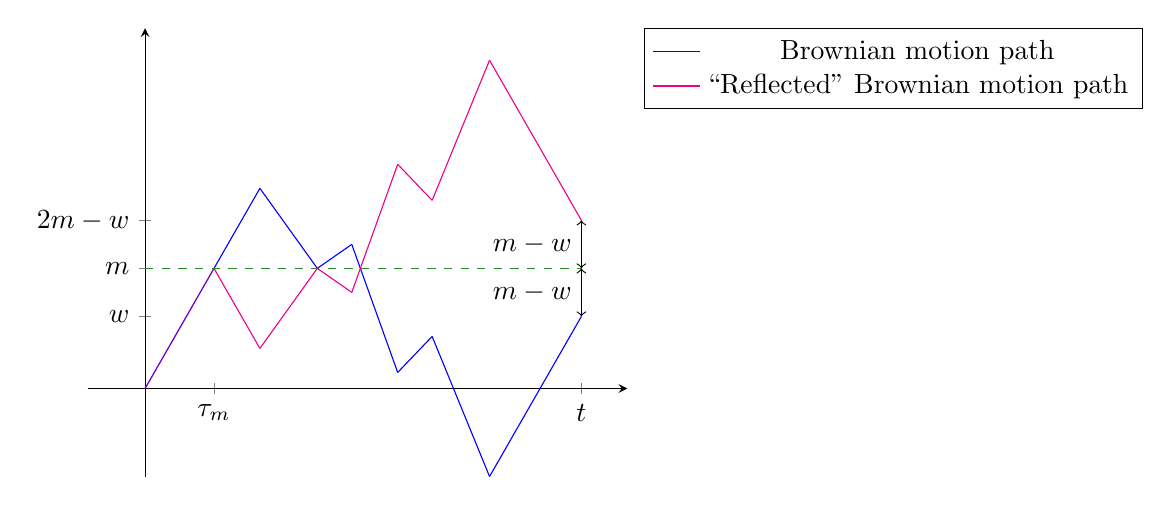
\begin{tikzpicture}
\begin{axis}[domain=-0.5:4, xmax=4.2, ymax=9, axis lines=middle, ytick=\empty,
xtick={0.6,3.8}, xticklabels={\(\tau_m\), \(t\)}, ytick={3, 1.8, 4.2},
yticklabels={\(m\), \(w\), \(2m-w\)}, legend pos=outer north east]
\addplot[blue, domain=0:1]{5*x};
\addplot[magenta, domain=0.6:1]{6-5*x};
\addlegendentry{Brownian motion path}
\addlegendentry{``Reflected'' Brownian motion path}
\addplot[magenta, opacity=0.5, domain=0:0.6]{5*x};
\addplot[draw=none, domain=-0.5:0]{x};
\addplot[blue, domain=1:1.5]{9-4*x};
\addplot[blue, domain=1.5:1.8]{2*x};
\addplot[blue, domain=1.8:2.2]{18-8*x};
\addplot[blue, domain=2.2:2.5]{0.4+3*(x-2.2)};
\addplot[blue, domain=2.5:3]{1.3-7*(x-2.5)};
\addplot[blue, domain=3:3.8]{-2.2+5*(x-3)};
\addplot[ForestGreen, domain=0:3.8, dashed]{3};
\addplot[magenta, domain=1:1.5]{-3+4*x};
\addplot[magenta, domain=1.5:1.8]{6-2*x};
\addplot[magenta, domain=1.8:2.2]{-12+8*x};
\addplot[magenta, domain=2.2:2.5]{5.6-3*(x-2.2)};
\addplot[magenta, domain=2.5:3]{4.7+7*(x-2.5)};
\addplot[magenta, domain=3:3.8]{8.2-5*(x-3)};
\draw[<->] (3.8,4.2) --node[midway, left]{\(m-w\)} (3.8,3);
\draw[<->] (3.8,3) --node[midway, left]{\(m-w\)} (3.8,1.8);
\end{axis}
\end{tikzpicture}
\end{center}
For every \blc{Brownian motion path of type \(1\)} (i.e., reaching level \(m\)
before time \(t\) but locating at a level \(w<m\) at time \(t\)), there would
be a corresponding \mgc{``reflected'' path} (due to the symmetry of Brownian
motion) that is at the level \(2m-w\) at time \(t\), which coincides with the
\blc{original path} at or before time \(\tau_m\), and is a mirror image of the
\blc{original path} about the line \(y=m\) after time \(\tau_m\).

Applying this argument repetitively to numerous paths, the ``number'' of paths
that reach level \(m\) before time \(t\) and locate at a level \(\le w\) at
time \(t\) would ``equal'' the ``number'' of paths that are at or above the
level \(2m-w\) at time \(t\). Therefore, intuitively, it is of equal
probability to have a path realized from any one of these types. This leads to
the \emph{reflection equality}.
\begin{theorem}[Reflection equality]
\label{thm:reflection-equality}
Let \(m>0\), \(\{W_t\}\) be a Brownian motion, and \(\tau_{m}\) be the first
passage time to level \(m\). Then, for every \(w\le m\), we have
\[
\blc{\prob{\tau_{m}\le t, W_t\le w}}=\mgc{\prob{W_t\ge 2m-w}}.
\]
\end{theorem}
\begin{pf}
Omitted.
\end{pf}
\item \textbf{Distribution and density functions of first passage time.} Using
the reflection equality, we can deduce the \emph{distribution function} and
\emph{density function} of the first passage time \(\tau_{m}\) (with \(m\ne
0\)), serving as tools for characterizing its distribution uniquely.
\begin{proposition}
\label{prp:first-pass-time-dist-dens-fun}
Let \(m\ne 0\) and \(\tau_{m}\) be the first passage time. Then:
\begin{enumerate}
\item The distribution function of \(\tau_{m}\) is
\[
\prob{\tau_{m}\le t}=\frac{2}{\sqrt{2\pi}}\int_{|m|/\sqrt{t}}^{\infty}e^{-y^{2}/2}\odif{y},
\quad t\ge 0.
\]
\item The density function of \(\tau_{m}\) is
\[
f_{\tau_{m}}(t)=\frac{|m|}{t\sqrt{2\pi t}}e^{-m^{2}/(2t)}, \quad t>0.
\]
\end{enumerate}
\end{proposition}
\begin{pf}
\begin{enumerate}
\item Consider first the case where \(m>0\). With \(w=m\) in
\Cref{thm:reflection-equality}, we get \(
\prob{\tau_{m}\le t, W_t< m}
=\prob{\tau_{m}\le t, W_t\le m}=\prob{W_t\ge m}\). Also, noting that \(W_t\ge
m\implies \tau_{m}\le t\), we have \(\prob{\tau_{m}\le t, W_t\ge
m}=\prob{W_t\ge m}\). Adding the two equations together then yields
\begin{align*}
\prob{\tau_m\le t}&=2\prob{W_t\ge m}
=\frac{2}{\sqrt{2\pi t}}\int_{m}^{\infty}\underbrace{e^{-x^{2}/(2t)}}
_{\text{pdf of \(\ndist{0,t}\)}}\odif{t} \\
\overset{\text{(substitution: \(y=x/\sqrt{t}\))}}&{=}
\frac{2}{\sqrt{2\pi}}\int_{m/\sqrt{t}}^{\infty}e^{-y^{2}/2}\odif{y}
=\frac{2}{\sqrt{2\pi}}\int_{|m|/\sqrt{t}}^{\infty}e^{-y^{2}/2}\odif{y}
.
\end{align*}
Next, for the case where \(m<0\), since \(\tau_m\) and \(\tau_{|m|}=\tau_{-m}\)
have the same distribution, the distribution function of \(\tau_{m}\) is
\[
\prob{\tau_{m}\le t}
=\prob{\tau_{-m}\le t}
\overset{(-m>0)}{=}\frac{2}{\sqrt{2\pi}}\int_{|-m|/\sqrt{t}}^{\infty}e^{-y^{2}/2}\odif{y}.
\]
\item Differentiating the distribution function from (a) with respect to \(t\)
gives
\begin{align*}
f_{\tau_{m}}(t)&=\odv{}{t}\frac{2}{\sqrt{2\pi}}\int_{|m|/\sqrt{t}}^{\infty}e^{-y^{2}/2}\odif{y}
\underset{\text{(chain rule)}}{\overset{\text{(Fundamental theorem of calculus)}}{=}}
-\frac{2}{\sqrt{2\pi}}e^{-(|m|/\sqrt{t})^{2}/2}
\cdot \odv{}{t}\frac{|m|}{\sqrt{t}} \\
&=\frac{|m|}{t\sqrt{2\pi t}}e^{-m^{2}/(2t)}, \quad t>0.
\end{align*}
\end{enumerate}
\end{pf}
\item \textbf{Distributions of Brownian motion and its maximum.} Let
\(\{W_t\}\) be a Brownian motion.  For every \(t\ge 0\), the \defn{maximum to
date} (time \(t\)) for the Brownian motion is defined by \(M_t=\max_{0\le s\le t}W_s\).
Such random variable is helpful in analyzing barrier options, and hence we
would like to study its distributional behaviours. The following result
suggests the joint distribution and conditional distribution of Brownian motion
\(W_t\) and the maximum to date \(M_t\):
\begin{proposition}
\label{prp:bm-max-joint-cond-dist}
Let \(\{W_t\}\) be a Brownian motion and \(M_t\) be its maximum to date (time
\(t\)) for every \(t\ge 0\). Then, for every \(t>0\):
\begin{enumerate}
\item The joint density function of \((M_t,W_t)\) is
\[
f_{M_t,W_t}(m,w)=\frac{2(2m-w)}{t\sqrt{2\pi t}}e^{-(2m-w)^{2}/(2t)},\quad m>0,\; w<m.
\]
\item The conditional density function of \(M_t\) given \(W_t=w\) is
\[
f_{M_t|W_t}(m|w)=\frac{2(2m-w)}{t}e^{2m(m-w)/t},\quad m>0,\; w<m.
\]
\end{enumerate}
\end{proposition}
\begin{pf}
\begin{enumerate}
\item Fix any \(m>0\) and \(w\le m\). By
\labelcref{it:first-pass-max-min-relate}, we have \(M_t\ge m\) iff \(\tau_m\le
t\). Hence,
\[
\prob{M_t\ge m, W_t\le w}
=\prob{\tau_m\le t, W_t\le w}
\overset{\text{(\Cref{thm:reflection-equality})}}{=}
\prob{W_t\ge 2m-w}
=\frac{1}{\sqrt{2\pi t}}\int_{2m-w}^{\infty}e^{-z^{2}/(2t)}\odif{z}.
\]
Also, we have
\[
\prob{M_t\ge m, W_t\le w}=\int_{m}^{\infty}\int_{-\infty}^{w}f_{M_t,W_t}(x,y)\odif{y}\odif{x}.
\]
These imply that
\[
\int_{m}^{\infty}\int_{-\infty}^{w}f_{M_t,W_t}(x,y)\odif{y}\odif{x}
=\frac{1}{\sqrt{2\pi t}}\int_{2m-w}^{\infty}e^{-z^{2}/(2t)}\odif{z}.
\]
Differentiating both sides with respect to \(m\) gives
\[
-\int_{-\infty}^{w}f_{M_t,W_t}(m,y)\odif{y}
=-\frac{2}{\sqrt{2\pi t}}e^{-(2m-w)^{2}/(2t)}.
\]
Next, differentiating both sides with respect to \(w\) gives
\[
f_{M_t,W_t}(m,w)
=\frac{2(2m-w)}{t\sqrt{2\pi t}}e^{-(2m-w)^{2}/(2t)},\quad m>0,\; w<m.
\]
\item By definition, we have
\begin{align*}
f_{M_t|W_t}(m|w)&=\frac{f_{M_t,W_t}(m,w)}{f_{W_t}(w)}
=\frac{2(2m-w)e^{-(2m-w)^{2}/(2t)}/(t\sqrt{2\pi t})}
{\underbrace{e^{w^{2}/2t}/\sqrt{2\pi t}}_{\text{pdf of \(\ndist{0,t}\)}}} \\
&=\frac{2(2m-w)}{t}e^{-2m(m-w)/t}
,\quad m>0,\; w<m.
\end{align*}
\end{enumerate}
\end{pf}
\end{enumerate}
